%*
%* Seven Kingdoms: Ancient Adversaries
%*
%* Copyright 1997,1998 Enlight Software Ltd.
%* Copyright 2018 Timothy Rink
%*
%* This program is free software: you can redistribute it and/or modify
%* it under the terms of the GNU General Public License as published by
%* the Free Software Foundation, either version 2 of the License, or
%* (at your option) any later version.
%*
%* This program is distributed in the hope that it will be useful,
%* but WITHOUT ANY WARRANTY; without even the implied warranty of
%* MERCHANTABILITY or FITNESS FOR A PARTICULAR PURPOSE.  See the
%* GNU General Public License for more details.
%*
%* You should have received a copy of the GNU General Public License
%* along with this program.  If not, see <http://www.gnu.org/licenses/>.
%*
%*

% bug here. image clipping

\chapter{Nationalities}

Nationalities differ not only in language and costume, but also in fighting skills and methods.

The Soldiers of all nationalities are well trained in the use of Basic Weapons, which are used for close-in fighting.

Some will acquire the skill of Ranged Weapons only after long years of training and the raising of their Combat Levels. Ranged weapons will then be used as a weapon of first choice. When, however, the enemy closes to fight at melee range, Soldiers will switch back to their Basic Weapons.

Others are expert in defenses that can turn a blade or arrow.

Others will, from time to time, become Berserkers and inflict great damage with a single stroke. This will happen at a set interval---but only with units that have been very well trained.

Below you will find a list of the abilities of each nationality.

\clearpage

\section{Chinese}

Long known for their skills in the martial arts, your Chinese Warriors will give you a well balanced and devastating attack. Striking like serpents with their Long Axes, they are also easily trained as archers who will kill from afar.

\begin{wrapfigure}{r}{0.5\textwidth}
	\begin{center}
		\vspace{-20pt}
		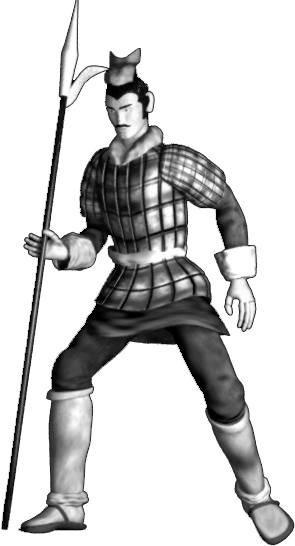
\includegraphics[width=0.3\textwidth]{Achinese}
	\end{center}
	\vspace{-20pt}
\end{wrapfigure}

Basic Weapon: Chinese Long Axe
\begin{adjustwidth}{1cm}{}
	Damage: 6–16 \\
	Delay between strokes: 2
\end{adjustwidth}
Ranged Weapon: Bow and Arrow
\begin{adjustwidth}{1cm}{}
	Damage: 5–8 \\
	Combat Level required: 30 \\
	Shot Delay: 7 \\ \\ \\ \\ \\ \\ \\ \\ 
\end{adjustwidth}

\begin{center}
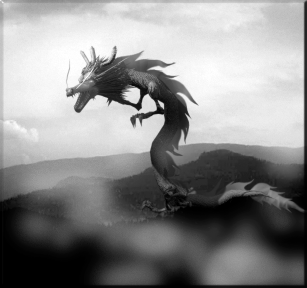
\includegraphics[width=74.25mm]{Ajingnung}
\includegraphics[width=74.25mm]{Ichinesehouse}
\end{center}

\clearpage

\section{Greeks}

The Greek Warrior excels in quick, sharp sword thrusts from behind the safety of his shield. From childhood, he is well schooled in the art of war. Training will introduce no new skills---but will greatly reinforce old ones.

\begin{wrapfigure}{r}{0.5\textwidth}
	\begin{center}
		\vspace{-20pt}
		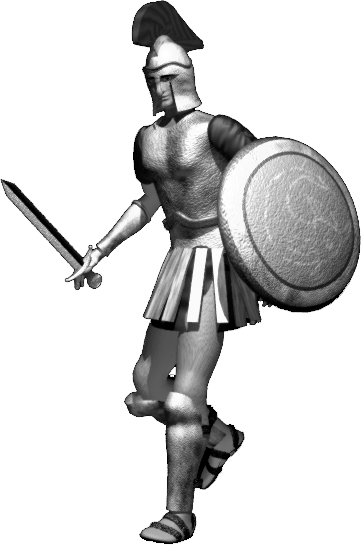
\includegraphics[width=0.3\textwidth]{Agreek}
	\end{center}
	\vspace{-20pt}
\end{wrapfigure}

Basic Weapon: Short Sword
\begin{adjustwidth}{1cm}{}
	Damage: 5–8 \\
	Delay between strokes: 1
\end{adjustwidth}
Basic Defense: Shield
\begin{adjustwidth}{1cm}{}
	The shield will completely block arrows from one direction only. \\ \\ \\ \\ \\ \\ \\ \\ 
\end{adjustwidth}

\begin{center}
	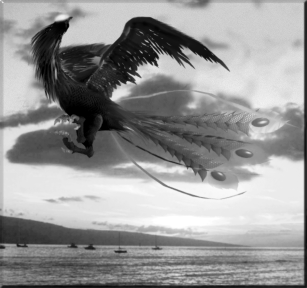
\includegraphics[width=74.25mm]{Aphoenix}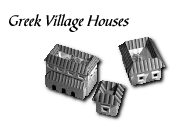
\includegraphics[width=74.25mm]{Igreekhouse}
\end{center}

\clearpage

\section{Japanese}

The Japanese Warrior is a fast-attacking and skilled swordsman. When the blood lust is upon him, a well trained warrior may dispatch an enemy with a single stroke.

\begin{wrapfigure}{r}{0.5\textwidth}
	\begin{center}
		\vspace{-20pt}
		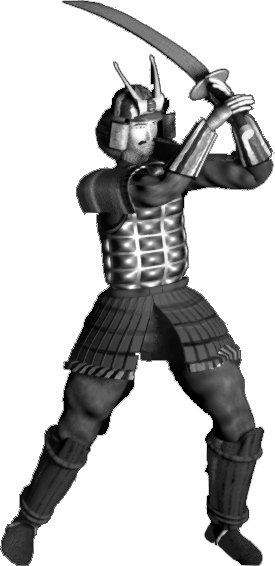
\includegraphics[width=0.3\textwidth]{Ajapanese}
	\end{center}
	\vspace{-20pt}
\end{wrapfigure}

Basic Weapon: Katana
\begin{adjustwidth}{1cm}{}
	Damage: 5–8 \\
	Delay between strokes: 2
\end{adjustwidth}
Berserker Attack: Katana
\begin{adjustwidth}{1cm}{}
	Damage: 32 \\
	Combat level required: 55 \\
	Stroke Delay: 90 \\ \\ \\ \\ \\ \\ \\ \\ 
\end{adjustwidth}

\begin{center}
	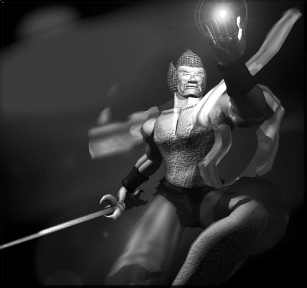
\includegraphics[width=74.25mm]{Amindturner}
\includegraphics[width=74.25mm]{Ijapanesehouse}
\end{center}

\clearpage

\section{Maya}

Wielding his Jaguar Fang club with incredible skill and power, the Mayan Warrior is devastating in close combat.

\begin{wrapfigure}{r}{0.5\textwidth}
	\begin{center}
		\vspace{-20pt}
		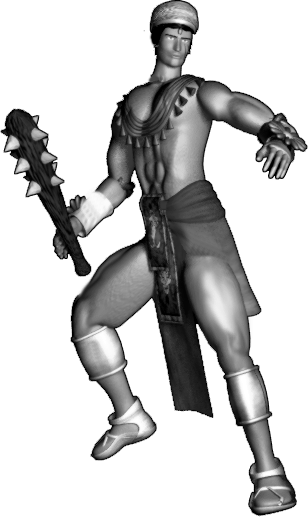
\includegraphics[width=0.3\textwidth]{Amaya}
	\end{center}
	\vspace{-20pt}
\end{wrapfigure}

Basic Weapon: Jaguar Fang Club
\begin{adjustwidth}{1cm}{}
	Damage: 8–14 \\
	Delay between strokes: 3 \\ \\ \\ \\ \\ \\ \\ \\ 
\end{adjustwidth}

\begin{center}
	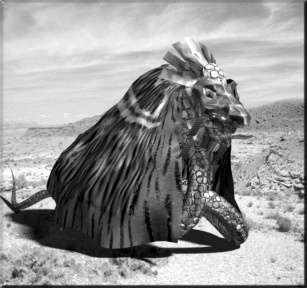
\includegraphics[width=74.25mm]{Akukulcan}
\includegraphics[width=74.25mm]{Imayanhouse}
\end{center}

\clearpage

\section{Normans}

The Norman Warrior’s value is in his versatility. Apart from his trusty Broadsword, a well trained Norman will protect himself with his shield and rain devastation from a distance with bolts from his crossbow.

\begin{wrapfigure}{r}{0.5\textwidth}
	\begin{center}
		\vspace{-20pt}
		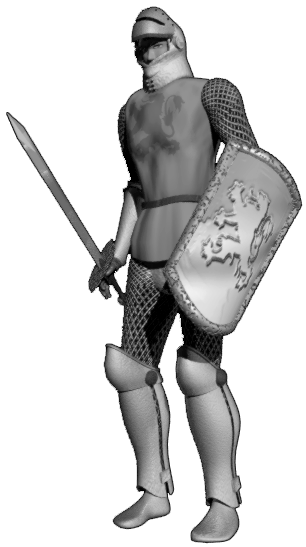
\includegraphics[width=0.3\textwidth]{Anorman}
	\end{center}
	\vspace{-20pt}
\end{wrapfigure}

Basic Weapon: Broadsword
\begin{adjustwidth}{1cm}{}
	Damage: 5–10 \\
	Delay between strokes: 3
\end{adjustwidth}
Ranged Weapon: Crossbow
\begin{adjustwidth}{1cm}{}
	Damage: 7–10 \\
	Combat level required: 50 \\
	Delay between shots: 8
\end{adjustwidth}
Defense: Shield
\begin{adjustwidth}{1cm}{}
	Will block all arrows from one direction only. \\
	Combat Level required: 30 
\end{adjustwidth}

\begin{center}
	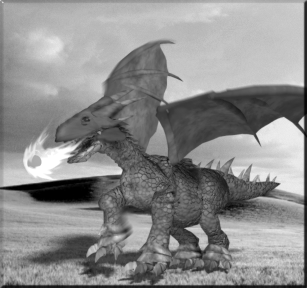
\includegraphics[width=74.25mm]{Adragon}
\includegraphics[width=74.25mm]{Inormanhouse}
\end{center}

\clearpage

\section{Persians}

Persians are born archers. Unlike the soldiers of other nations, who must be trained in the use of the bow, your Persian Warriors will enter your service already skilled in this weapon.

For close-in work, they will fight with their spears, although not with great skill.

\begin{wrapfigure}{r}{0.5\textwidth}
	\begin{center}
		\vspace{-20pt}
		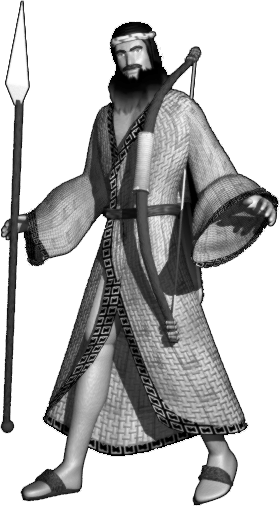
\includegraphics[width=0.3\textwidth]{Apersian}
	\end{center}
	\vspace{-20pt}
\end{wrapfigure}

Basic Weapon: Spear
\begin{adjustwidth}{1cm}{}
	Damage: 3–6 \\
	Delay between strokes: 3
\end{adjustwidth}
Basic Ranged Weapon: Bow and Arrow
\begin{adjustwidth}{1cm}{}
	Damage: 6–12 \\
	Shot Delay: 6 \\ \\ \\ \\ \\ \\ \\ \\ 
\end{adjustwidth}

\begin{center}
	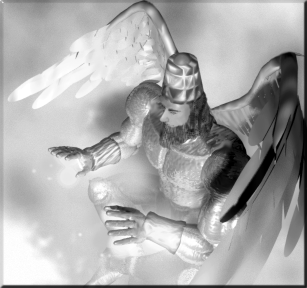
\includegraphics[width=74.25mm]{Ahealinglord}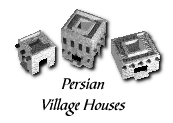
\includegraphics[width=74.25mm]{Ipersianhouse}
\end{center}

\clearpage

\section{Vikings}

Your Vikings are hard-swinging, hard-fighting warriors, ideal for close-in and dirty butchery.

When well trained, they will occasionally go berserk and wreak havoc in enemy ranks.

\begin{wrapfigure}{r}{0.5\textwidth}
	\begin{center}
		\vspace{-20pt}
		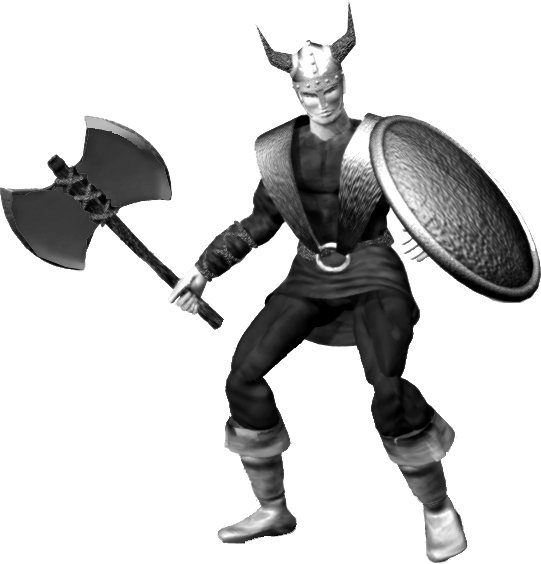
\includegraphics[width=0.3\textwidth]{Aviking}
	\end{center}
	\vspace{-20pt}
\end{wrapfigure}

Basic Weapon: Heavy Axe
\begin{adjustwidth}{1cm}{}
	Damage: 6–12 \\
	Delay between strokes: 4
\end{adjustwidth}
Berserker Attack: Lightning Axe
\begin{adjustwidth}{1cm}{}
	Lightning Axe will inflict greater damage on enemy units. \\
	Damage: 40 \\
	Combat level required: 50 \\
	Stroke Delay: 120 
\end{adjustwidth}

\begin{center}
	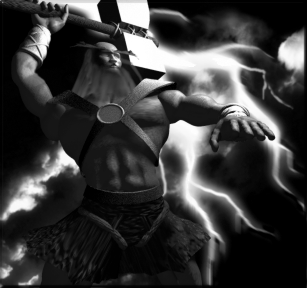
\includegraphics[width=74.25mm]{Athor}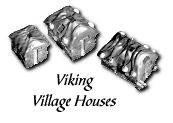
\includegraphics[width=74.25mm]{Ivikinghouse}
\end{center}

\clearpage

\section{Egyptians}

With his fighting traditions dating back over 3,000 years, your Egyptian warrior is a master of many skills.

\begin{wrapfigure}{r}{0.5\textwidth}
	\begin{center}
		\vspace{-20pt}
		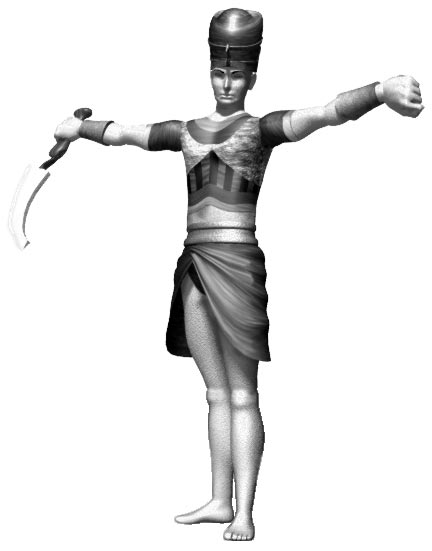
\includegraphics[width=0.3\textwidth]{Aegyptian}
	\end{center}
	\vspace{-20pt}
\end{wrapfigure}

Basic Weapon: Khopesh
\begin{adjustwidth}{1cm}{}
	Damage: 5–9 \\
	Delay between slashes: 3
	\end{adjustwidth}
Range Attack: Bow and Arrow
\begin{adjustwidth}{1cm}{}
	Damage: 6-9 \\
	Combat level required: 40 \\
	Shot Delay: 7
\end{adjustwidth}
Power Attack: Ra Arrows
\begin{adjustwidth}{1cm}{}
	Damage: 25 \\
	Combat level required: 70
	Shot Delay: 120 
\end{adjustwidth}

\begin{center}
	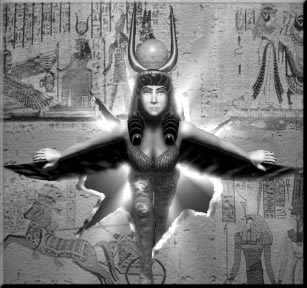
\includegraphics[width=74.25mm]{Aisis}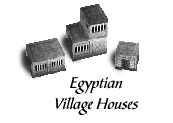
\includegraphics[width=74.25mm]{Iegyptianhouse}
\end{center}

\clearpage

\section{Mughuls}

With their scimitars flashing in the blazing sun, your Mughul warriors will cleave through enemy ranks like a desert wind.

\begin{wrapfigure}{r}{0.5\textwidth}
	\begin{center}
		\vspace{-20pt}
		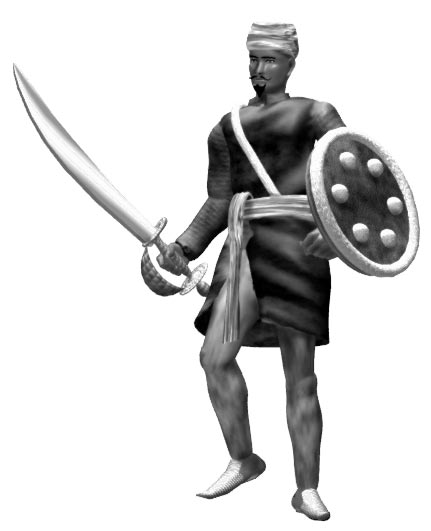
\includegraphics[width=0.3\textwidth]{Amughal}
	\end{center}
	\vspace{-20pt}
\end{wrapfigure}

Basic Weapon: Scimitar
\begin{adjustwidth}{1cm}{}
	Damage: 5–11 \\
	Delay between strokes: 3
\end{adjustwidth}
Berserker Attack: Scimitar
\begin{adjustwidth}{1cm}{}
	Damage: 30 \\
	Combat level required: 60 \\
	Stroke Delay: 100 \\ \\ \\ \\ \\ \\ \\ \\ 
\end{adjustwidth}

\begin{center}
	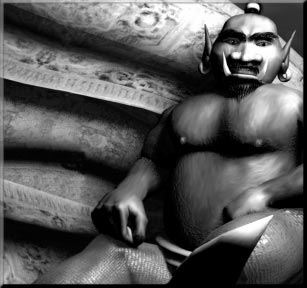
\includegraphics[width=74.25mm]{Adjinni}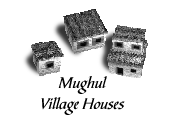
\includegraphics[width=74.25mm]{Imughalhouse}
\end{center}

\clearpage

\section{Zulus}

Rising up from the tall grasses, your Zulu warrior will rain down a devastating shower of spears upon any who dare to invade his lands.
	
\begin{wrapfigure}{r}{0.5\textwidth}
	\begin{center}
		\vspace{-20pt}
		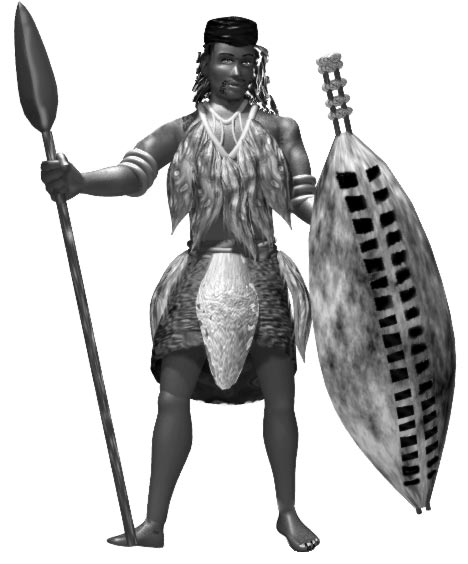
\includegraphics[width=0.3\textwidth]{Azulu}
	\end{center}
	\vspace{-20pt}
\end{wrapfigure}

Basic Weapon: Assegai
\begin{adjustwidth}{1cm}{}
	Damage: 4–7 \\
	Delay between thrusts: 3
\end{adjustwidth}
Range Weapon: Throwing Spear
\begin{adjustwidth}{1cm}{}
	Damage: 10–18 \\
	Delay between throws: 15 \\
	Combat level required: 30
\end{adjustwidth}
Defense: Shielding against range attacks when not throwing spear
\begin{adjustwidth}{1cm}{}
	Combat level required: 50
\end{adjustwidth}

\begin{center}
	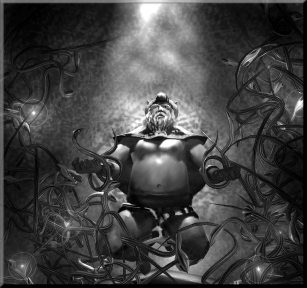
\includegraphics[width=74.25mm]{Aoldone}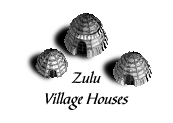
\includegraphics[width=74.25mm]{Izuluhouse}
\end{center}